% This is the second main part of the thesis. The experiments should be suitable to validate your approach.
% Define the experimental setting, e.g. the robot or the dataset, the metrics as well as the results.
% The visualization of the results should be in a way such that it is easily understandable.
% Usually, first, the results are reported and then the effects of the results on the defined problem are discussed.
% Answer the question, what parts of the problem did you solve?
\chapter{Experiments}
\label{chap:experiments}

In order to compare our different approaches we measured the time an iteration of our control loop takes.
This allows us to compare not only the speed of each program version but also the consistency in the iteration times.

\section{Methodology}
\label{sec:experiments:methodology}

In order to make the benchmarks as comparable as possible we set a few invariants between the runs:
\begin{itemize}
  \item Each of the benchmarks is run on the exact same RaspberryPi 4B.
  \item The Pi runs at the stock core frequency of 1800MHz.
  \item The linux versions run RaspberryPi OS, a derivative of Debian Linux with the stock configuration.
  \item The kernel version is 6.1.73 for the stock and isolated core versions.
  \item The realtime version runs on 6.1.73-rt which was compiled prior on the RaspberryPi. For Instructions to replicate this kernel see the Appendix \ref{sec:appendix:realtime}.
  \item Our control loop target value is set to a constant for these tests and the IC-MU position encoder is fixed in place in order to return almost the same value each iteration.
  \item Rustc 1.79.0 was used for all rust builds, both native and cross compiled to bare-metal
  \item GCC 13.2.1 was used as the cross compiler as well as linker for compiling the Circle library and linking it to the Rust code.
  \item GCC 12.2.0 was used as the native linker for the Rust code.
\end{itemize}

\subsection{Testing the linux based versions}
The linux versions all run a common iteration function:
\begin{lstlisting}[language=Rust,style=colouredRust]
  pub fn iteration(...) -> Instant {
      // fetch step: calculate elapsed time, get new position and setpoint
      let iteration_time = last_iteration_start.elapsed();
      let iteration_start = Instant::now();
  
      let position = get_position(spi);
      let setpoint = get_setpoint();
  
      // compute step: calculate new output value
      pid.setpoint = setpoint;
      let output = pid
          .step(pid_ctrl::PidIn::new(position, iteration_time.as_secs_f64()))
          .out;
  
      // update step: output the new value over PWM
      pwm.set_duty_cycle(output).unwrap();
  
      iteration_start
  }
\end{lstlisting}

Time measurment is done here through Rusts stdlib Instant and Duration types.
On linux these compile to the clock\_gettime syscall in order to get microsecond accurate time.
Because the RaspberryPi 4 does not yet have a real time clock like the Raspberry Pi 5,
linux uses the clock interrupts of a 1MHz oscillator to measure the time.
The benchmarks are first run for 10000 iterations without measuring, in order to avoid any latency spikes because of cache missess in the real benchmark.
The real benchmark is then run for 1000000 iterations while saving the measured time deltas to an array.
To execute the benchmarks the criterion framework for Rust was used as it allows easy configuration of the amount of samples,
runs an unmeasured three second warmup loop of the benchmark beforehand and automatically generates plots and statistics data from the results.

For the isolated core version we use the cset python program in order to easily manipulate the linux kernels cpuset subsystem.
This allows us with few commands to isolate one core from all running processess and run our program on it, without being disturbed by core local interrupts.
Global interrupts such as spinlocks when running a syscall can however still halt our execution flow.

We can run cset from inside of our program with the current process id this way:
\begin{lstlisting}[language=Rust,style=colouredRust]
  Command::new("sudo")
      .args([
          "cset",
          "shield",
          "--cpu=3",
          "--kthread=on",
          &format!("--pid={}", std::process::id()),
      ])
      .spawn()
      .expect("Could not start cset binary")
      .wait()
      .expect("cset did not exit successfully");
\end{lstlisting}

For the realtime version we needed a kernel that can boot with the Raspberry Pi bootloader,
have the out-of-tree kernel modules for spi and pwm and support fully preemtive scheduling.
In order to get that combination, the official sources for the Rpi kernel were patched with the fitting version of the PREEMP\_RT patchset and compiled.

To achieve this Step 1 is to get all the required build dependencies.
\begin{lstlisting}[language=bash, breaklines]
  sudo apt update && sudo apt install build-essential flex bison libssl-dev bc
\end{lstlisting}

Step 2 is to get the kernel sources and patch them with the correct PREEMPT-RT patchset.
\begin{lstlisting}[language=bash, breaklines]
  wget https://github.com/raspberrypi/linux/archive/refs/tags/stable_20240124.tar.gz
  wget https://cdn.kernel.org/pub/linux/kernel/projects/rt/6.1/older/patch-6.1.73-rt22.patch.xz
  tar -xf stable_20240124.tar.gz
  cd linux-stable_20240124
  xzcat ../patch-6.1.73-rt22.patch.xz | patch -p1
\end{lstlisting}

Step 3 is to generate the kernel config, we use the provided default config for the Raspberry Pi 4 and only set the PREEMPT\_RT config value to enable full kernel preemption.
\begin{lstlisting}[language=bash, breaklines]
  make bcm2711_defconfig
  ./scripts/config -e PREEMPT_RT
  make olddefconfig
\end{lstlisting}

Step 4 is to actually compile the kernel, this takes about 3 hours on all 4 cores of the Raspberry Pi 4.
\begin{lstlisting}[language=bash, breaklines]
  make -j4 Image.gz modules dtbs
\end{lstlisting}

Step 5 is to actually install the files.
\begin{lstlisting}[language=bash, breaklines]
  sudo make modules_install
  sudo cp arch/arm64/boot/dts/broadcom/*.dtb /boot/firmware/
  sudo cp arch/arm64/boot/dts/overlays/*.dtb* /boot/firmware/overlays/
  sudo cp arch/arm64/boot/dts/overlays/README /boot/firmware/overlays/
  sudo cp arch/arm64/boot/Image.gz /boot/firmware/kernel8.img
\end{lstlisting}

At the end reboot to load the new kernel.

\subsection{Testing the bare-metal version}
Benchmarking the bare-metal version is a bit more involved than the linux based versions.
For measuring times Circle's CTimer::GetClockTicks64() is used. This in turn returns the amount of ticks of the 1MHz oscillator on the Rpi.
Analogous to the linux versions the loop is run for 10000 iterations before we start measuring.

The second difficulty with the bare-metal version is getting the results out of the RaspberryPi.
We need to either transmit the data over a connection such as ethernet, spi, i2c to another PC or save it to a filesystem on removable storage.
Since we are running bare-metal that means we need a driver for one of these options.
Because we are already using the Circle library for Spi and it provides simple access to a USB mass storage device with a FAT32 file system we will be using it to save the results.

The process for this is equivalent to how we already used the SPI and PWM drivers in the \nameref{chap:concept_and_implementation} chapter,
so we will only skim over the most important parts.

In our wrapper.hpp we need to include "circle/fs/fat/fatfs.h" and "circle/usb/usbhcidevice.h"
\begin{lstlisting}[language=C++]
#include "circle/fs/fat/fatfs.h"
#include "circle/usb/usbhcidevice.h"
\end{lstlisting}

In our main.rs we initialize these devices and save the measured times as a csv file.
\begin{lstlisting}
let mut usb_hci =
    ffi::CXHCIDevice::new(&mut interrupt_system, &mut timer, false, 0, null_mut());
let mut filesystem = ffi::CFATFileSystem::new();


((*usb_hci._base._base.vtable_).CUSBController_Initialize)(&mut usb_hci._base._base, true);

for _ in 0..10000 {
    ...
}
const N: usize = 200;
let mut times = [0; N];
for time in times.iter_mut() {
    ...
    *time = ffi::CTimer::GetClockTicks64() - iteration_start;
    ...
    iteration_start = ffi::CTimer::GetClockTicks64();
    ...
}

let partition = device_name_service.GetDevice(c"umsd1-1".as_ptr(), true);
filesystem.Mount(partition);

let file = filesystem.FileCreate(c"times.csv".as_ptr());
let mut buffer = String::from("iteration,elapsed_time_us\n");
for (n, time) in times.iter().enumerate() {
    buffer.push_str(&format!("{},{}\n", n, time));
}
let buffer = alloc::ffi::CString::new(buffer).unwrap();

filesystem.FileWrite(
    file,
    buffer.as_ptr() as *const c_void,
    buffer.count_bytes() as u32,
);
filesystem.FileClose(file);
filesystem.UnMount();
\end{lstlisting}

\section{Results}
\label{sec:experiments:results}

Now for the actual measurments.
In our simplest case we look at some statistical data from the measurments.
Most important for our purposes are the average and worst case times.

\begin{table}[h!]
  \label{tab:measurments}
  \begin{tabular}{|l|l|l|l|l|}
    \hline
                   & Mean    & Min  & Max    & Std Dev \\ \hline
    bare-metal     & 4.4us   & 4us  & 7us    & 0.49us  \\ \hline
    linux-default  & 40.38us & 39us & 876us  & 11.53us \\ \hline
    linux-isolated & 40.11us & 38us & 2200us & 12.29us \\ \hline
    linux-rt       & 53.35us & 51us & 2507us & 25.59us \\ \hline
  \end{tabular}
\end{table}

To better visualize this and better understand the behavior of any outliers we have depicted the iteration times both in a histogram as well as the raw data points.
The iteration time graphs allow for a better understanding of the relative difference between a normal iteration and the outlier ones,
but due to the amount of datapoints obscure how often or rare these outlier actually occur.
In order to overcome this downside we have the histogram with a logarithmic scale

\makeatletter
\newcommand{\includesvggraphics}[2][\textwidth]{
  \filename@parse{#2}%
  \includesvg[inkscapepath=svg-inkscape/\filename@area,width=#1]{#2}
}
\makeatother

\begin{figure}
  \begin{center}
    \begin{minipage}{0.48\textwidth}
      \begin{center}
        \includesvggraphics{assets/bare-metal/hist.svg}
        \caption{Histogram of the iteration times for one million iterations of the bare-metal version}
        \label{fig:experiments:bare-metal:hist}
      \end{center}
    \end{minipage}
    \hspace{0.02\textwidth}
    \begin{minipage}{0.48\textwidth}
      \begin{center}
        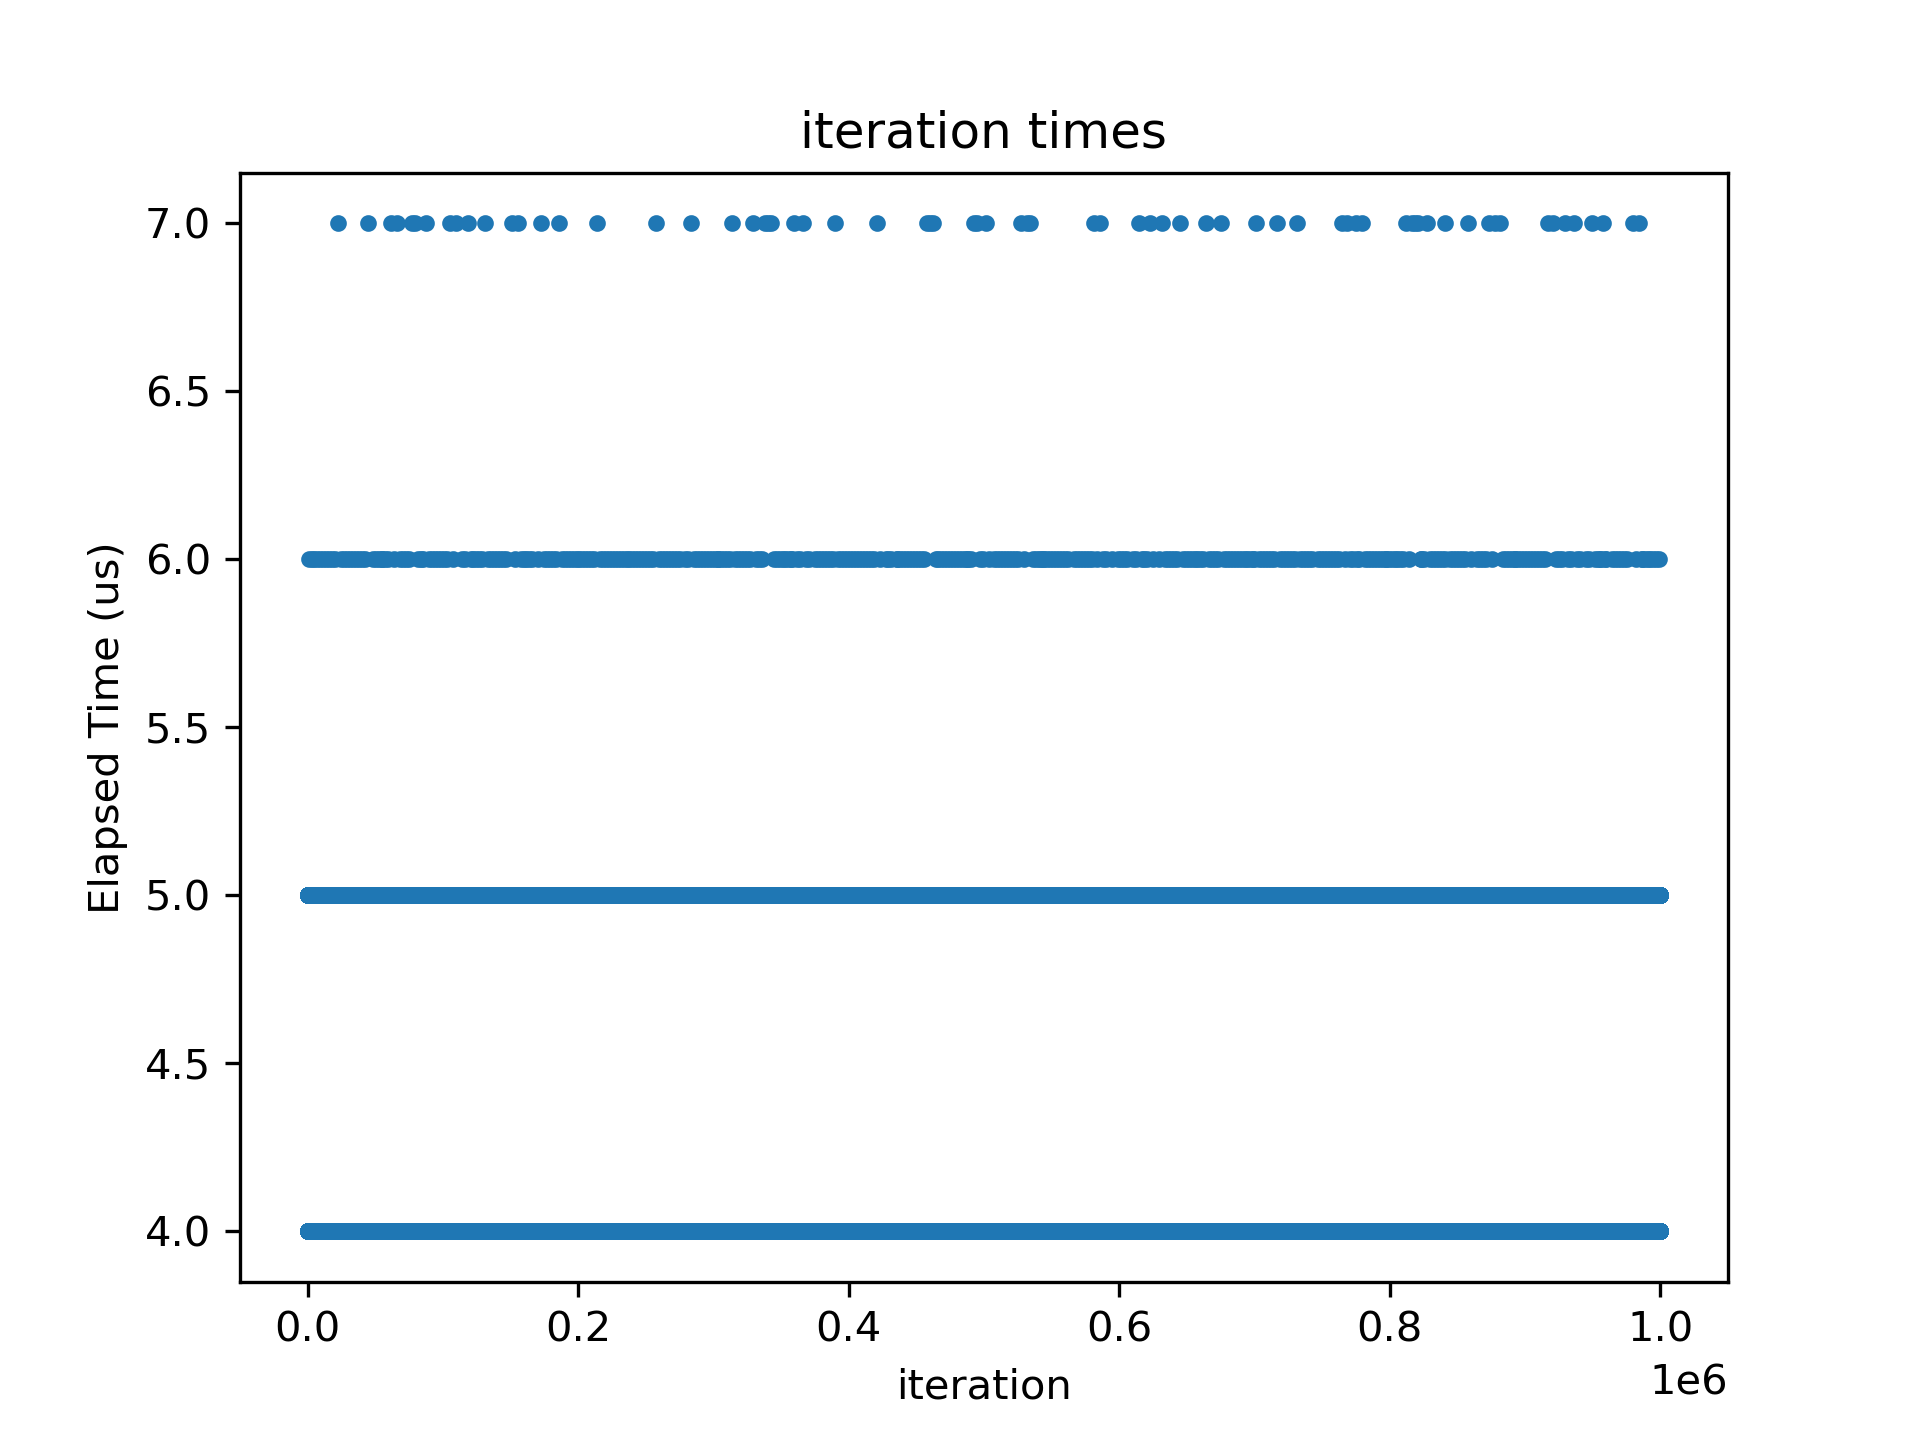
\includegraphics[width=\textwidth]{assets/bare-metal/times.png}
        \caption{The iteration time of every iteration in chronologic order for the bare-metal version}
        \label{fig:experiments:bare-metal:times}
      \end{center}
    \end{minipage}
  \end{center}
\end{figure}

\begin{figure}
  \begin{center}
    \begin{minipage}{0.48\textwidth}
      \begin{center}
        \includesvggraphics{assets/os-default/hist.svg}
        \caption{Histogram of the iteration times for one million iterations of the linux version without any modifications}
        \label{fig:experiments:os-default:hist}
      \end{center}
    \end{minipage}
    \hspace{0.02\textwidth}
    \begin{minipage}{0.48\textwidth}
      \begin{center}
        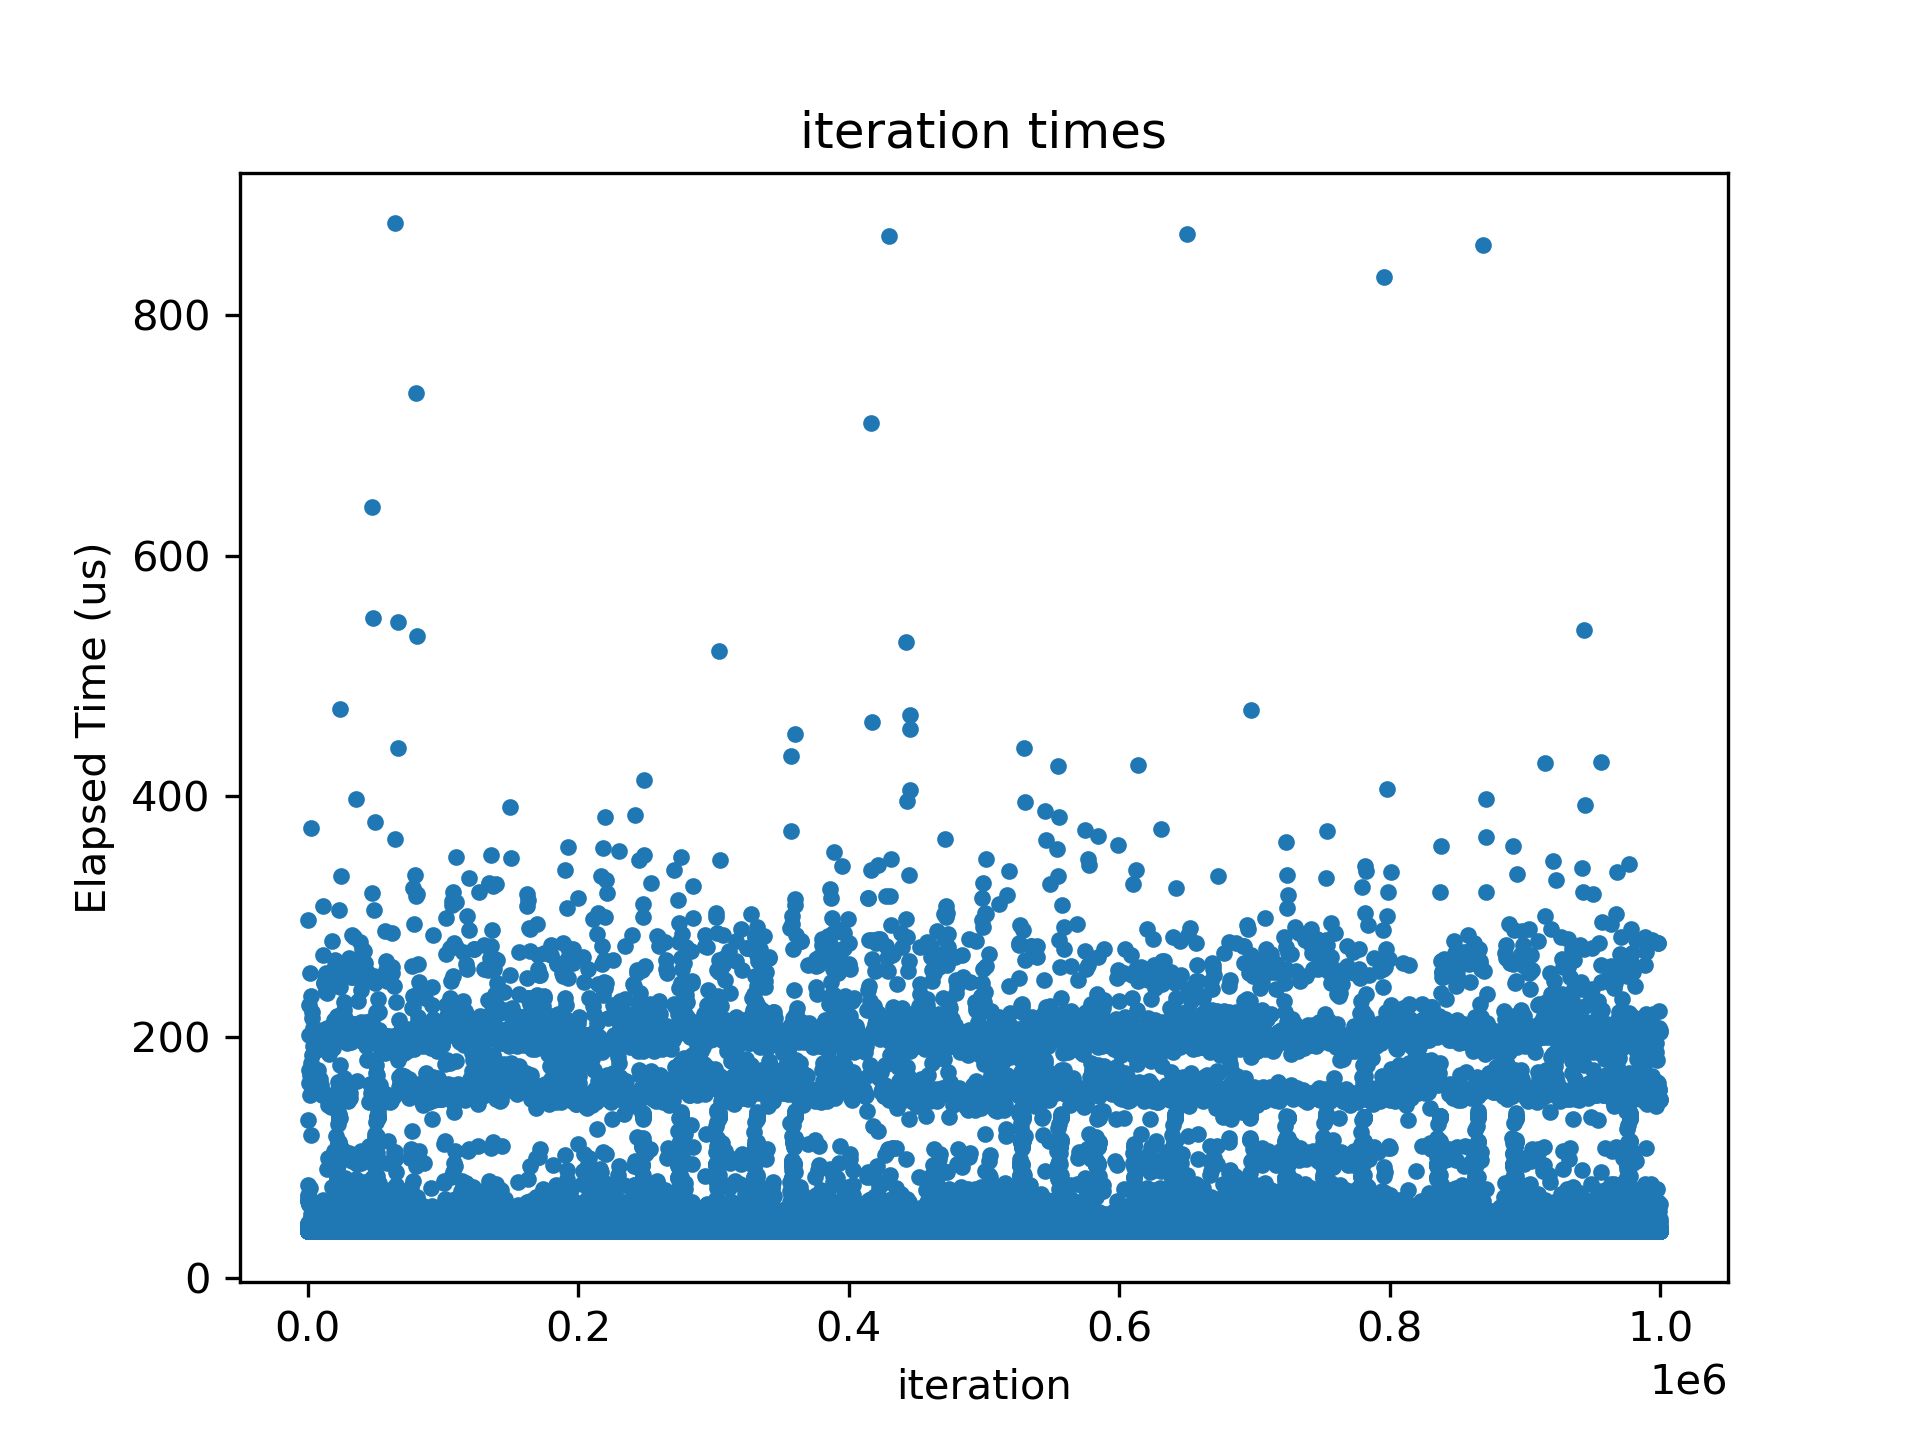
\includegraphics[width=\textwidth]{assets/os-default/times.png}
        \caption{The iteration time of every iteration in chronologic order for the linux version without any modifications}
        \label{fig:experiments:os-default:times}
      \end{center}
    \end{minipage}
  \end{center}
\end{figure}

\begin{figure}
  \begin{center}
    \begin{minipage}{0.48\textwidth}
      \begin{center}
        \includesvggraphics{assets/os-isolated/hist.svg}
        \caption{Histogram of the iteration times for one million iterations of the linux version on a reserved core}
        \label{fig:experiments:os-isolated:hist}
      \end{center}
    \end{minipage}
    \hspace{0.02\textwidth}
    \begin{minipage}{0.48\textwidth}
      \begin{center}
        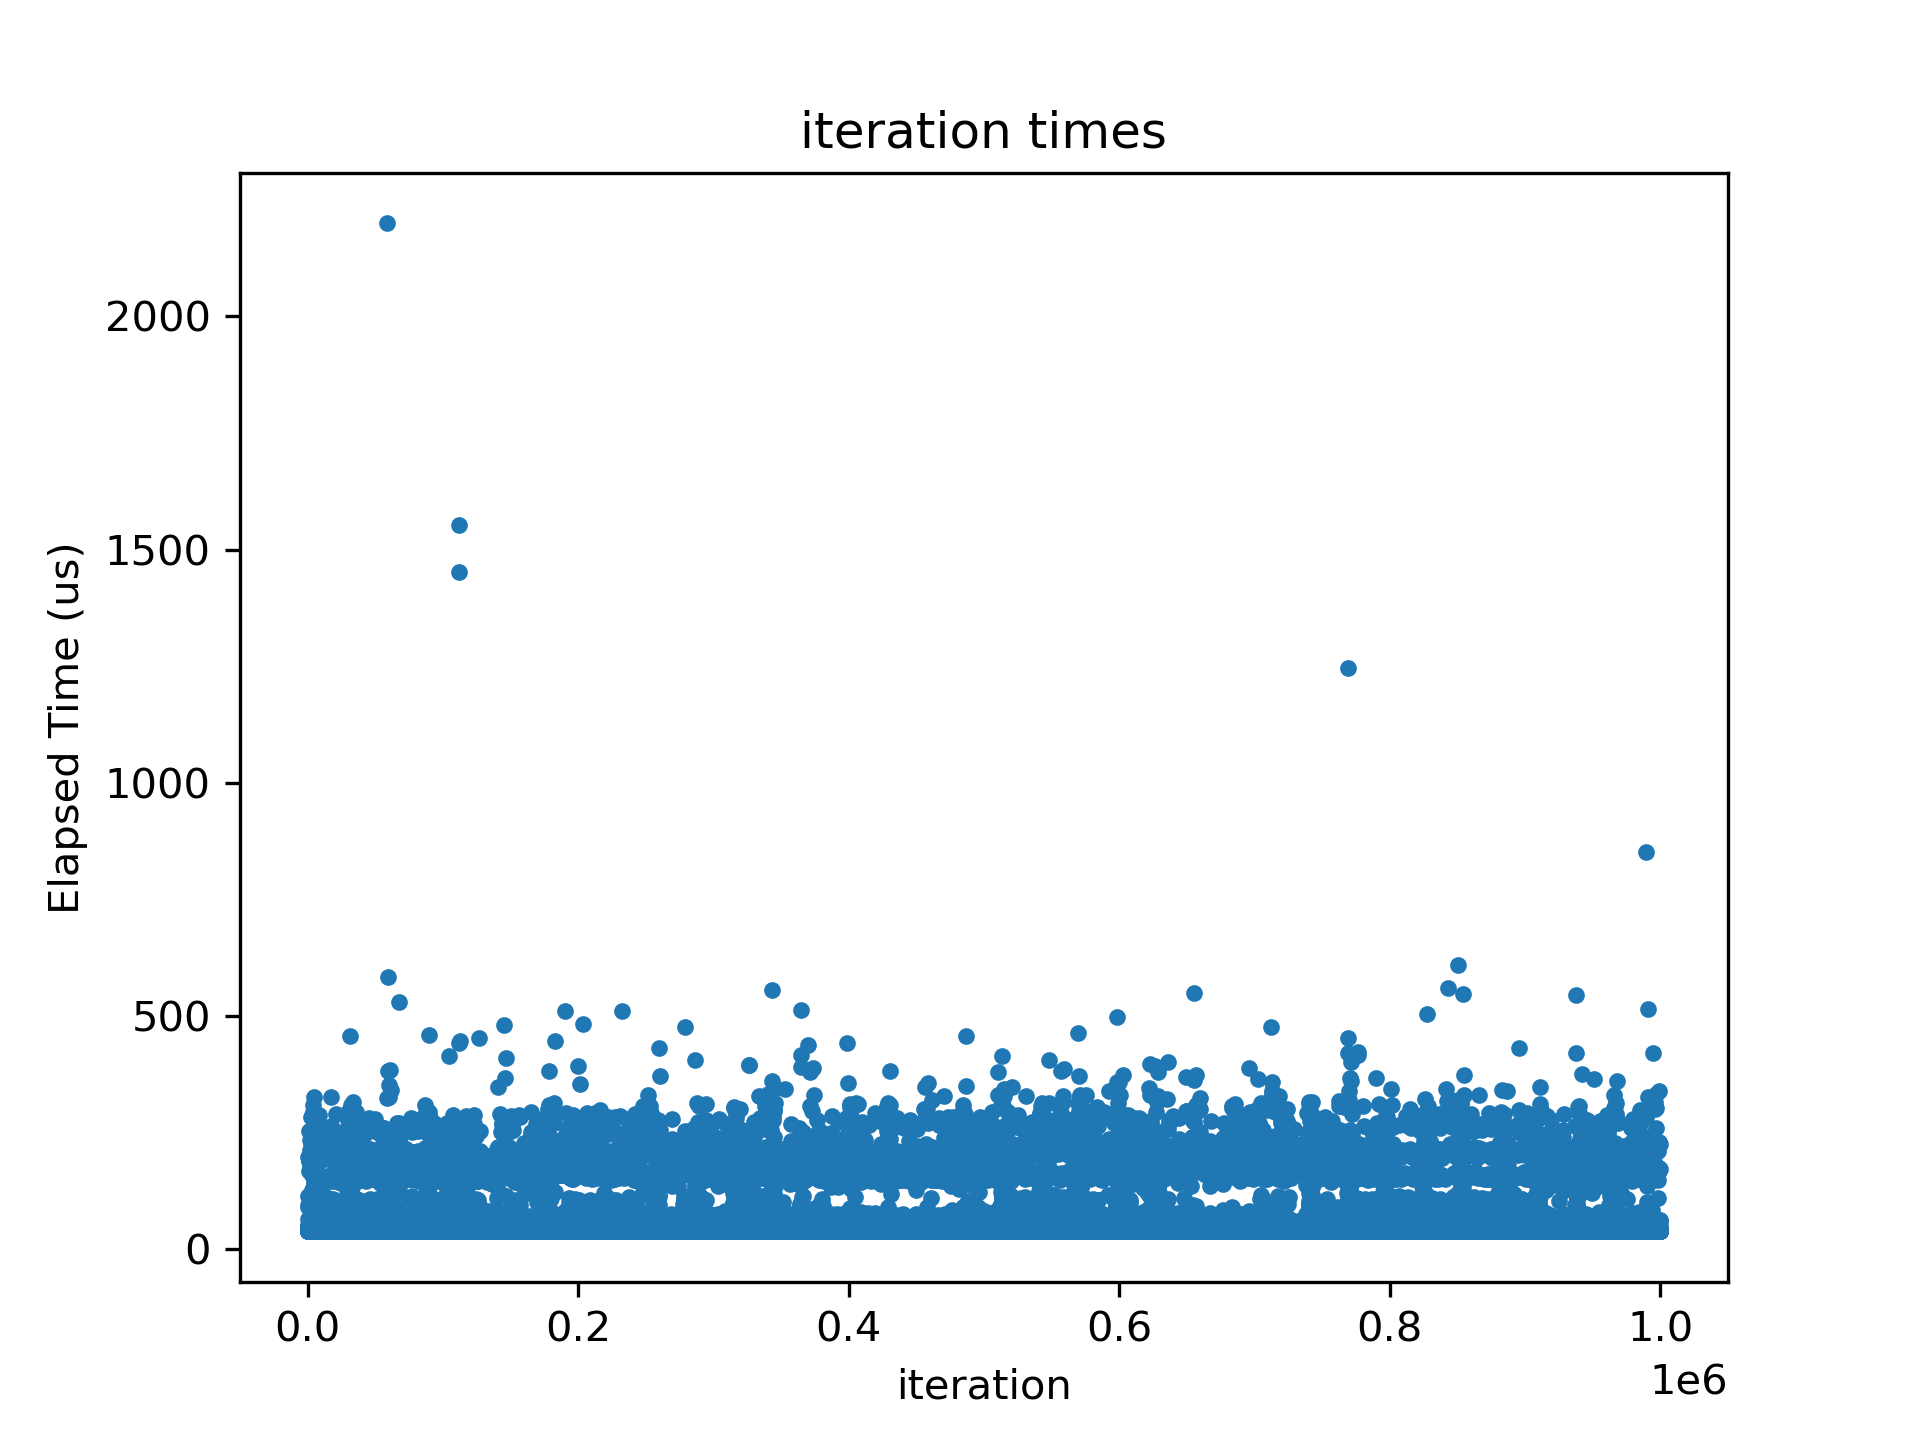
\includegraphics[width=\textwidth]{assets/os-isolated/times.png}
        \caption{The iteration time of every iteration in chronologic order for the linux version on a reserved core}
        \label{fig:experiments:os-isolated:times}
      \end{center}
    \end{minipage}
  \end{center}
\end{figure}

\begin{figure}
  \begin{center}
    \begin{minipage}{0.48\textwidth}
      \begin{center}
        \includesvggraphics{assets/os-rt/hist.svg}
        \caption{Histogram of the iteration times for one million iterations of the linux version with a realtime kernel}
        \label{fig:experiments:os-rt:hist}
      \end{center}
    \end{minipage}
    \hspace{0.02\textwidth}
    \begin{minipage}{0.48\textwidth}
      \begin{center}
        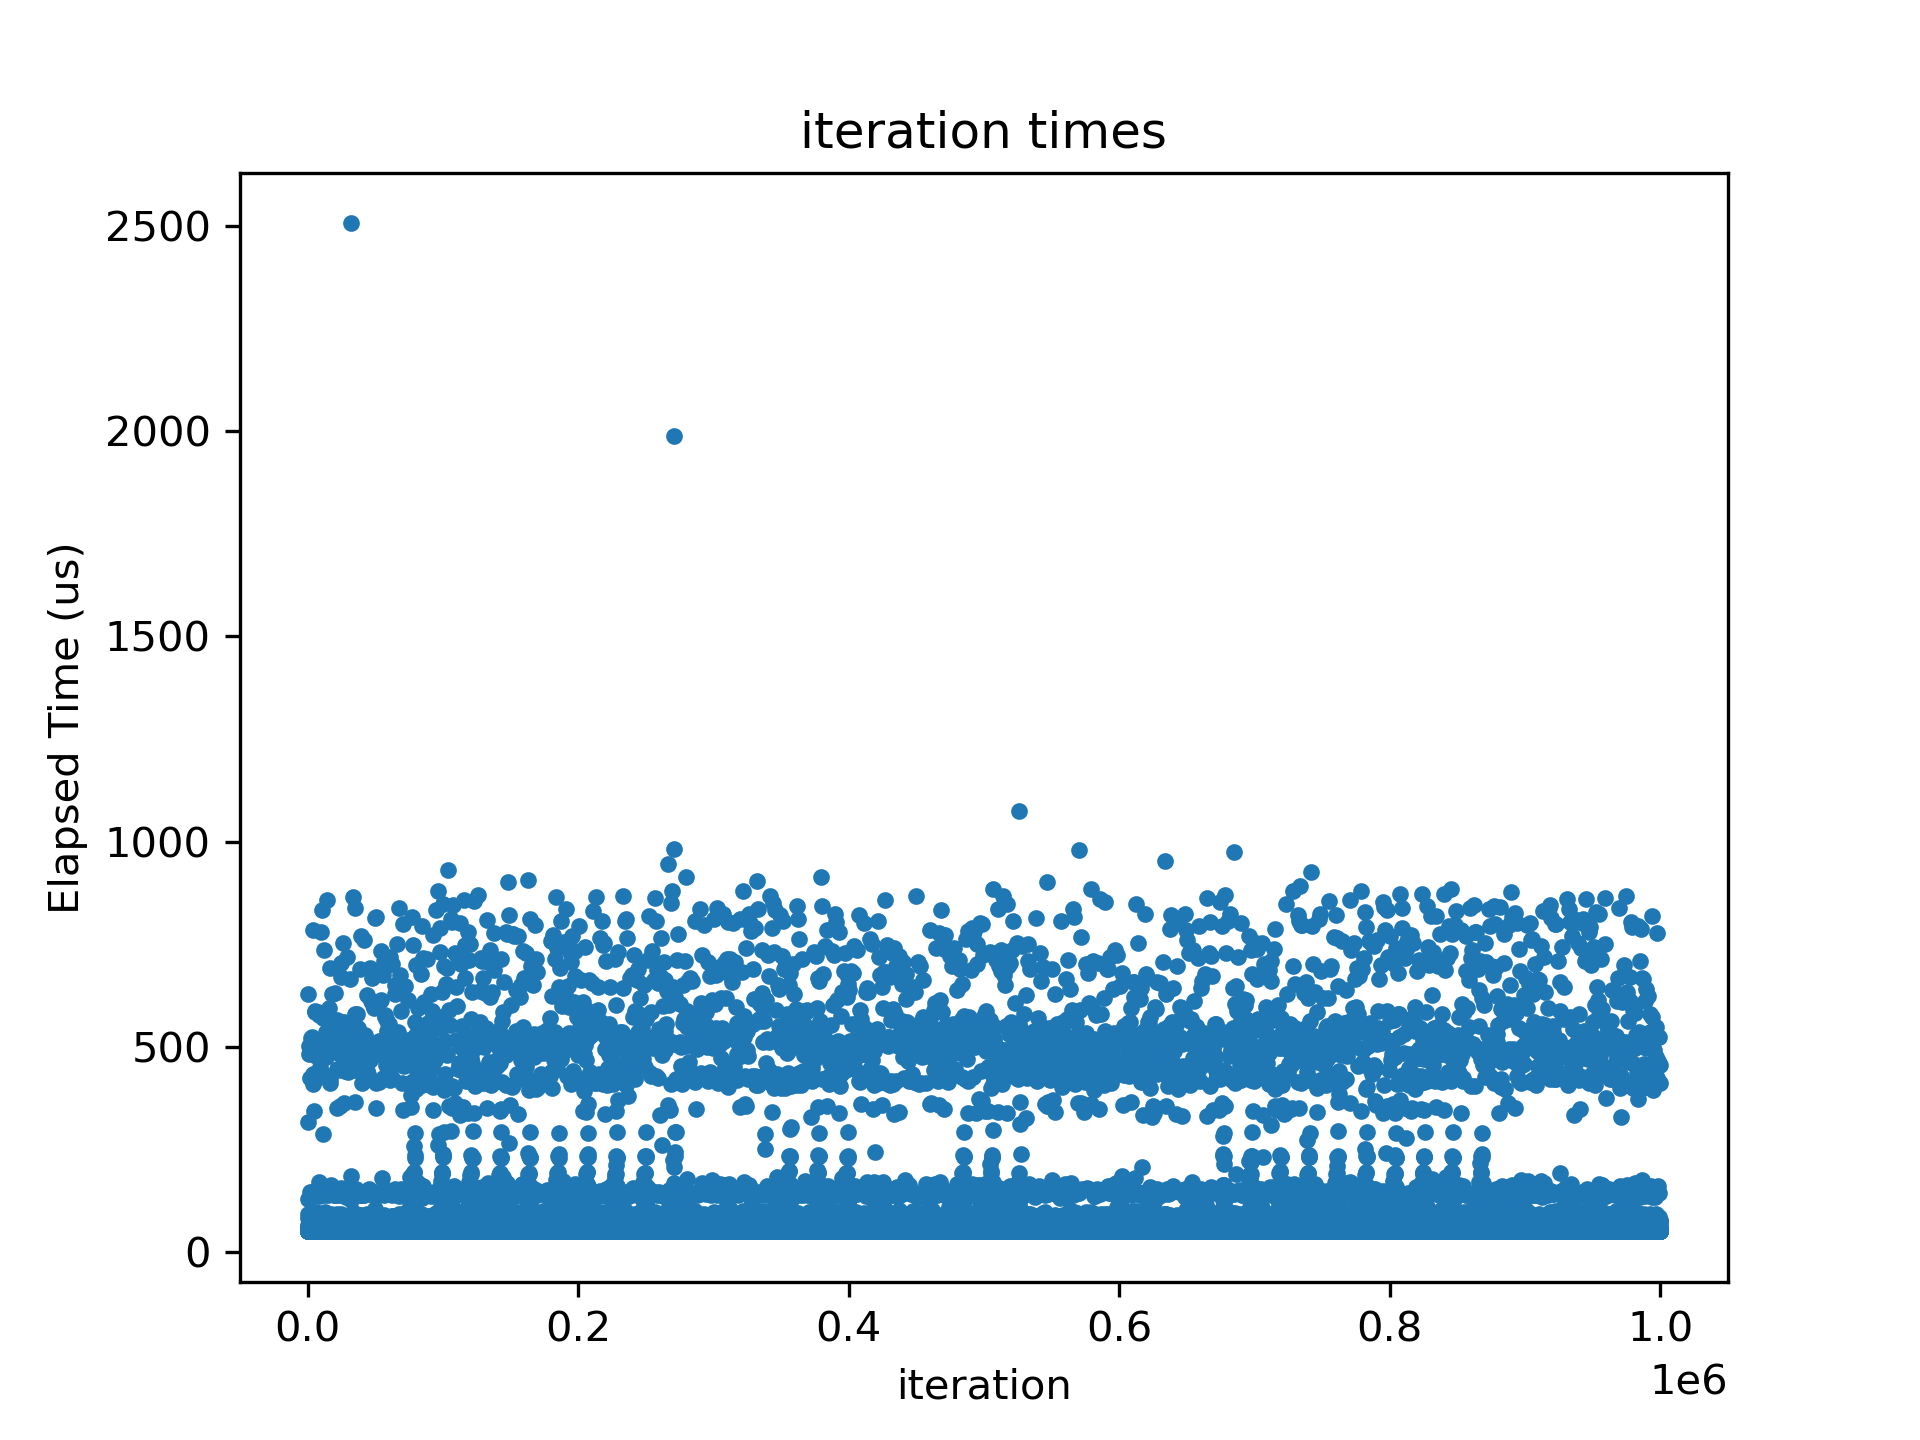
\includegraphics[width=\textwidth]{assets/os-rt/times.png}
        \caption{The iteration time of every iteration in chronologic order for the linux version with a realtime kernel}
        \label{fig:experiments:os-rt:times}
      \end{center}
    \end{minipage}
  \end{center}
\end{figure}

\section{Interpretation}

There are two different things here to analyze.
First, the difference between the bare-metal and linux version.
All of the linux based versions have average execution times of an order of magnitude more than the bare-metal version,
which leaves the question:
Is this speed difference adequately explained by the linux version having to switch the execution context to the kernel and back for the PWM and SPI kernel drivers?
To answer this properly, we profiled a run of the default linux version, the result can be seen in \ref{fig:experiments:flamegraph}.
From this we can see that most of the time (84.12\%) is spent setting the duty cycle, which in turn means that the context switching overhead is not the issue.
If it was, we would see close to the same duration for SPI and getting the system time, as we see for PWM.
This can have one of two causes:\\
The linux kernel PWM driver is very slow.
Or, the rppal implementation of set\_duty\_cycle() is not optimal,
either because it does extra steps not needed for our case,
or talks to the kernel in an inefficient way.
Of these two the second one is more likely for two reasons,
code in the linux kernel gets significantly more exposure and testing than rppal and the Circle PWM source code states,
that it is heavily inspired by the linux implementation.
If the reason is indeed that rppal could have been programmed differently for this task,
a significant speedup could be achieved.
Assuming the set\_duty\_cycle() was as fast as the SPI transfer,
which would be reasonable as the spi transfer has to write and read to memory and the duty cycle function only has to do one write,
the linux version times would come down to roughly 15us,
putting it in a very comparable ballpark as the bare-metal version.

\begin{figure}
  \begin{center}
    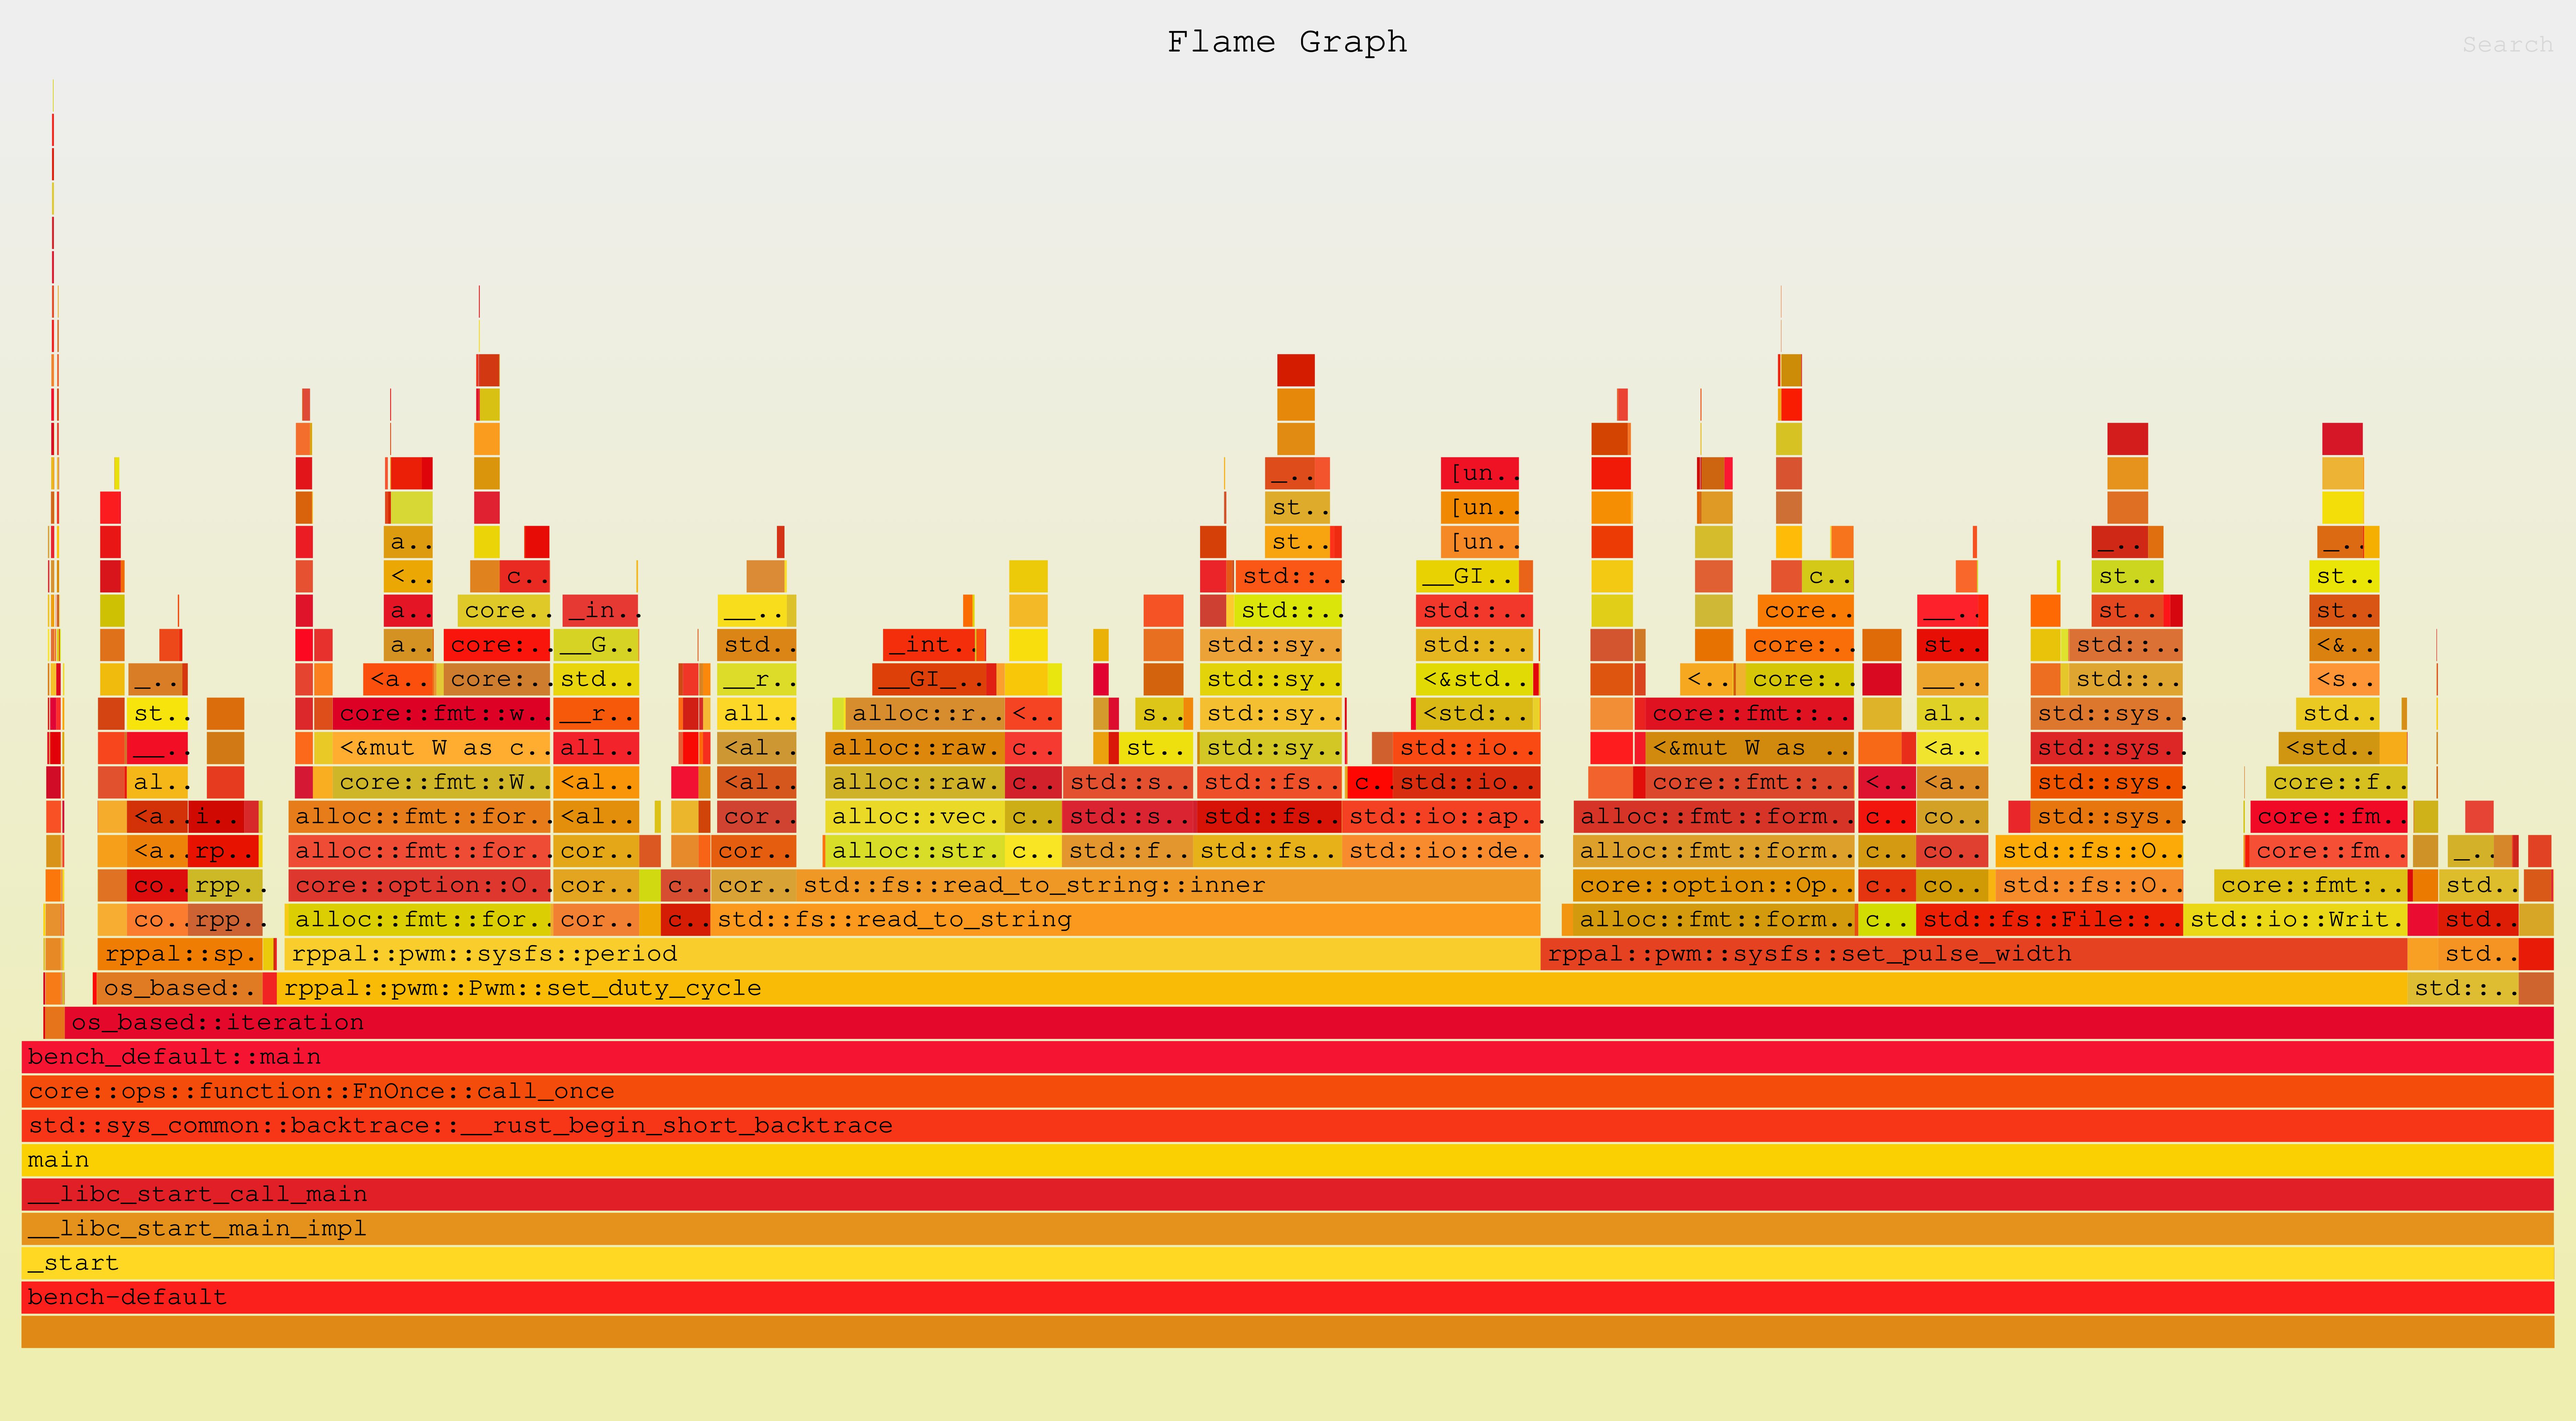
\includegraphics[width=\textwidth]{assets/os-default/flamegraph.png}
    \caption{A flamegraph for the default linux version, with times spent inside of each function}
    \label{fig:experiments:flamegraph}
  \end{center}
\end{figure}

The second part of the results that is worth analyzing is the comparison of the linux version with each other.
The goal of reducing the worst case latencies on linux has failed.
Every one of the linux versions has regular lag spikes to over an order of magnitude more than the average iteration time.
The isolated core and realtime versions that we hoped would reduce this behavior show very similar behavior as the stock version for iteration times under 1ms,
but additionally have rare spikes up in the 2-2.5ms region.

With both of these results in mind it is safe to say that the bare-metal version is the one more suited for the target application,
as regular reaction time spikes of almost a microsecond are just not acceptable and the lower average iteration times are preferable.
